% Options for packages loaded elsewhere
\PassOptionsToPackage{unicode}{hyperref}
\PassOptionsToPackage{hyphens}{url}
%
\documentclass[
]{article}
\usepackage{amsmath,amssymb}
\usepackage{lmodern}
\usepackage{iftex}
\ifPDFTeX
  \usepackage[T1]{fontenc}
  \usepackage[utf8]{inputenc}
  \usepackage{textcomp} % provide euro and other symbols
\else % if luatex or xetex
  \usepackage{unicode-math}
  \defaultfontfeatures{Scale=MatchLowercase}
  \defaultfontfeatures[\rmfamily]{Ligatures=TeX,Scale=1}
\fi
% Use upquote if available, for straight quotes in verbatim environments
\IfFileExists{upquote.sty}{\usepackage{upquote}}{}
\IfFileExists{microtype.sty}{% use microtype if available
  \usepackage[]{microtype}
  \UseMicrotypeSet[protrusion]{basicmath} % disable protrusion for tt fonts
}{}
\makeatletter
\@ifundefined{KOMAClassName}{% if non-KOMA class
  \IfFileExists{parskip.sty}{%
    \usepackage{parskip}
  }{% else
    \setlength{\parindent}{0pt}
    \setlength{\parskip}{6pt plus 2pt minus 1pt}}
}{% if KOMA class
  \KOMAoptions{parskip=half}}
\makeatother
\usepackage{xcolor}
\usepackage[margin=1in]{geometry}
\usepackage{graphicx}
\makeatletter
\def\maxwidth{\ifdim\Gin@nat@width>\linewidth\linewidth\else\Gin@nat@width\fi}
\def\maxheight{\ifdim\Gin@nat@height>\textheight\textheight\else\Gin@nat@height\fi}
\makeatother
% Scale images if necessary, so that they will not overflow the page
% margins by default, and it is still possible to overwrite the defaults
% using explicit options in \includegraphics[width, height, ...]{}
\setkeys{Gin}{width=\maxwidth,height=\maxheight,keepaspectratio}
% Set default figure placement to htbp
\makeatletter
\def\fps@figure{htbp}
\makeatother
\setlength{\emergencystretch}{3em} % prevent overfull lines
\providecommand{\tightlist}{%
  \setlength{\itemsep}{0pt}\setlength{\parskip}{0pt}}
\setcounter{secnumdepth}{-\maxdimen} % remove section numbering
\usepackage{booktabs}
\usepackage{longtable}
\usepackage{array}
\usepackage{multirow}
\usepackage{wrapfig}
\usepackage{float}
\usepackage{colortbl}
\usepackage{pdflscape}
\usepackage{tabu}
\usepackage{threeparttable}
\usepackage{threeparttablex}
\usepackage[normalem]{ulem}
\usepackage{makecell}
\usepackage{xcolor}
\ifLuaTeX
  \usepackage{selnolig}  % disable illegal ligatures
\fi
\IfFileExists{bookmark.sty}{\usepackage{bookmark}}{\usepackage{hyperref}}
\IfFileExists{xurl.sty}{\usepackage{xurl}}{} % add URL line breaks if available
\urlstyle{same} % disable monospaced font for URLs
\hypersetup{
  pdftitle={Eye-tracking data in A-FFIP (BOSCA battery)},
  hidelinks,
  pdfcreator={LaTeX via pandoc}}

\title{Eye-tracking data in A-FFIP (BOSCA battery)}
\author{}
\date{\vspace{-2.5em}2023-06-05}

\begin{document}
\maketitle

This is the state of the eye-tracking assessments in June 2023

\hypertarget{prepare-data-base-output}{%
\subsection{prepare data base output}\label{prepare-data-base-output}}

** load different data base output files ** caluclate test age based on
WPPSI or Bayley measures

\hypertarget{sympom-severity-in-sample}{%
\subsection{sympom severity in sample}\label{sympom-severity-in-sample}}

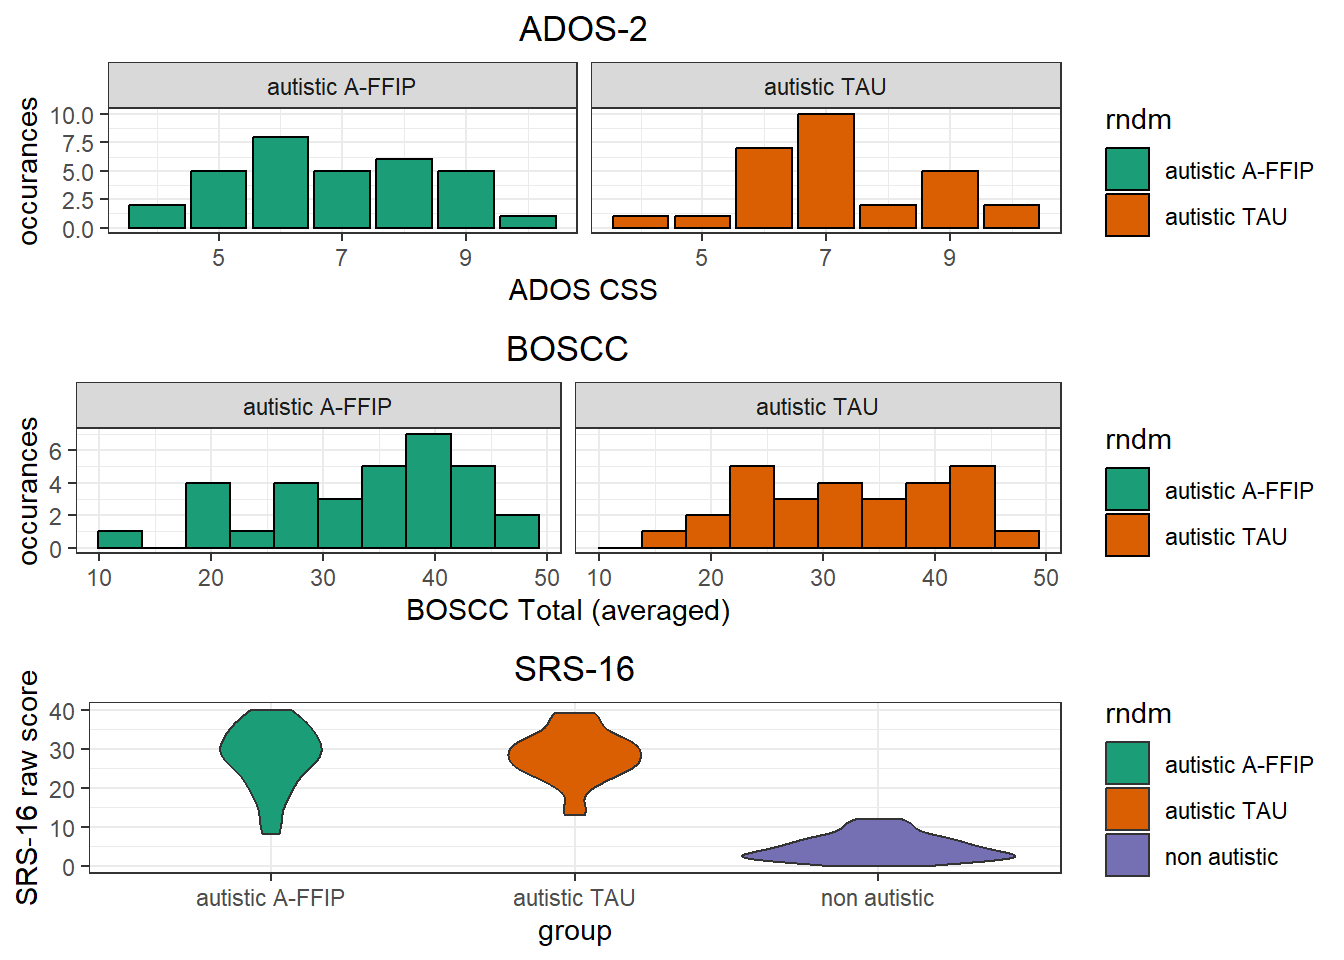
\includegraphics{sample_overview_June2023_files/figure-latex/visualize symptom severity-1.pdf}

\hypertarget{prepare-eye-tracking-data-quality-sheet}{%
\subsection{prepare eye-tracking data quality
sheet}\label{prepare-eye-tracking-data-quality-sheet}}

\begin{verbatim}
## 
## FALSE  TRUE 
##    24   141
\end{verbatim}

\begin{verbatim}
## 
## FALSE  TRUE 
##     4   298
\end{verbatim}

\begin{verbatim}
## 
##   T2   T4   T6  FU2  FU3    K K_FU 
##   67   58   53   20    4   69   29
\end{verbatim}

\hypertarget{data-visualization}{%
\subsection{Data Visualization}\label{data-visualization}}

\hypertarget{overview-of-assessment-quality}{%
\subsubsection{overview of assessment
quality}\label{overview-of-assessment-quality}}

\begin{verbatim}
## calib_quality
##    bad   else failed   good medium 
##     29     11     78    134     50
\end{verbatim}

\hypertarget{overview-of-the-assessments-by-asessment-dates}{%
\subsubsection{Overview of the assessments by asessment
dates}\label{overview-of-the-assessments-by-asessment-dates}}

\includegraphics{sample_overview_June2023_files/figure-latex/assessment dates-1.pdf}

\hypertarget{distribution-of-test-age-bayley-or-wppsi-compared-to-biological-age}{%
\subsubsection{Distribution of test age (Bayley or WPPSI) compared to
biological
age}\label{distribution-of-test-age-bayley-or-wppsi-compared-to-biological-age}}

\includegraphics{sample_overview_June2023_files/figure-latex/age data-1.pdf}

\end{document}
